\documentclass{article}
\usepackage[utf8]{inputenc}
\usepackage{siunitx}
\usepackage{graphics}
\usepackage[american,siunitx]{circuitikz}
\usepackage{amsmath}
\usepackage{svg}
\usepackage{booktabs}
\usepackage{float}
\usepackage{xparse, xfp}
\usepackage{graphicx} 
%\renewcommand{\thesubsection}{\thesection.\alph{subsection}}
\newcommand{\equal}{=}
\ExplSyntaxOn
\NewDocumentCommand{\defcon}{mm}
 {
  \cs_new:Npx #1 { \fp_eval:n { #2 } }
 }
\ExplSyntaxOff

\title{ECE2101L\\Electrical Circuit Analysis II Laboratory\\\,\\Lab 4\\Response of Source-free Parallel RLC Circuits\\\,\\Report\\}
\author{Choi Tim Antony Yung\\\,\\Willis Nguyen\\Phineas Cozmiuc}
\date{24 February 2020}

\begin{document}

\maketitle

\newpage


\section*{Objective}
The purpose of this experiment is to explore the behavior of a second order underdamped or overdamped parallel RLC circuit in absence of an external source.

\section{Underdamped Second Order Parallel RLC Circuit}
\begin{center}
    \begin{circuitikz}
        \draw 
            (0,0) -- (-2,0) to[voltage source, l_= $V_s$] (-2,-3) -- (0,-3)
            (0,0) 
            coordinate(R1) -- ++(2.25,0)
            coordinate(n1) -- ++(1.75,0)
            coordinate(L1) -- ++(1.75,0)
            coordinate(n2) -- ++(2.25,0)
            coordinate(C1)
            (R1) to[R=$R\equal\SI{3.3}{\kilo\ohm}$, i>^=$i_R$] ++(0,-3)
            (n1) ++(0,-0.25) to[open, v^=v] ++(0,-2.5)
            (L1) node[circ,label=v]{} to[L=$L\equal\SI{1}{\henry}$, i>^=$i_L\equal I_0$] ++(0,-3) node[ground]{}
            (n2) ++(0,-0.25) to[open, v^=v] ++(0,-2.5)
            (C1) to[C=$C\equal\SI{50}{\micro\farad}$, i>^=$i_c$, v=$v_c$] ++(0,-3) --(0,-3)
            ;
    \end{circuitikz}
\end{center}

The voltage response of the above RLC circuit can be represented by the differential equation below:

$$\frac{d^2v}{dt^2}+\frac{1}{RC}\frac{dv}{dt}+\frac{1}{LC}v=0$$
$$\frac{d^2v}{dt^2}+\frac{1}{(3.3\times10^3)(50\times10^{-6})}\frac{dv}{dt}+\frac{1}{(50\times10^{-6})}v=0$$
$$\frac{d^2v}{dt^2}+\frac{20}{33}\frac{dv}{dt}+20000\,v=0$$\\

The damping factor $\alpha$ and undamped natural frequency $\omega_0$ for the above parallel RLC circuit is the following:
$$\alpha = \frac{1}{2RC}=\frac{10}{33}\approx3.03$$
$$\omega_0 = \sqrt{\frac{1}{LC}}=100\sqrt{2}\approx 141.42$$\\

The condition for solution in underdamped, critically damped, and overdamped case in terms of $\alpha$ and $\omega_0$ is the following:
\[ \begin{cases} 
      \alpha < \omega_0 & underdamped \\
      \alpha = \omega_0 & critically\; damped \\
      \alpha > \omega_0 & overdamped 
   \end{cases}
\]\\

As $3.03\approx\alpha < \omega_0\approx141.42$, we can determine that the above circuit is an underdamped second order RLC circuit.\\

The characteristic equation in relation to the above differential equation is the following:
$$s^2+2\alpha s+\omega_0^2=0$$

Utilizing the quadratic equation, we can obtain the following expressions for determining the roots of the characteristic equation in terms of RLC and in terms of $\alpha$ and $\omega_0$:
$$s=-\alpha \pm\sqrt{\alpha^2-\omega_0^2}$$
$$s=-\alpha \pm j\sqrt{\omega_0^2-\alpha^2}$$\\

Let $\omega_d=\sqrt{\omega_0^2-\alpha^2}\approx 141.39$, then the general solution of v(t) is as follows:
$$v(t)=A_1e^{s_1t}+A_2e^{s_2t}$$
$$v(t)=e^{-\alpha t}(A_1e^{j\omega_dt}+A_2e^{-j\omega_dt})$$
$$v(t)=e^{-\alpha t}(A_1[cos(\omega_dt)+jsin(\omega_dt)]+A_2[cos(-\omega_dt)+jsin(-\omega_dt)])$$
$$v(t)=e^{-\alpha t}[(A_1+A_2)cos(\omega_dt)+j(A_1-A_2)sin(\omega_dt)]$$\\

Let $B_1=A_1+A_2$ and $B_2=j(A_1-A_2)$
$$v(t)=e^{-\alpha t}[B_1cos(\omega_dt)+B_2sin(\omega_dt)]$$\\

The initial condition v'(0) can be determined as follow with KCL at node v:
$$i_R+i_L+i_c=0$$
$$\frac{v}{R}+I_0+Cv'=0$$
$$v'=-\frac{\frac{v}{R}+I_0}{C}$$
$$v'(0)=-\frac{\frac{v(0)}{R}+I_0}{C}\approx -18.18$$\\


The coefficient $B_1$ and $B_2$ can then be calculated based on initial condition $v(0)$ and $v'(0)$ as follows:
$$v(0) =e^{-\alpha 0}[B_1cos(\omega_d0)+B_2sin(\omega_d0)] = B_1=3$$
$$v'(0) =e^{-\alpha 0}[(-\alpha B_1 + \omega_d B_2)cos(\omega_d0)+(-\omega_dB_1-\alpha B_2)sin(\omega_d0)]$$
$$v'(0)=-\alpha B_1 + \omega_d B_2$$
$$ B_2 = \frac{v'(0) + \alpha v(0)}{\omega_d} =-0.0643$$\\

The complete solution of v is the following:
$$v(t)=e^{-3.03 t}[3cos(141.39t)-0.0643sin(141.39t)]$$\\

As the circuit operated in absence of an external force, the above waveform demonstrated a natural response of the RLC circuit.\\

The following is the plot of $v(t)$ with MATLAB. The source code is appended at the end of this report.
\begin{figure}[H]
    \centering
        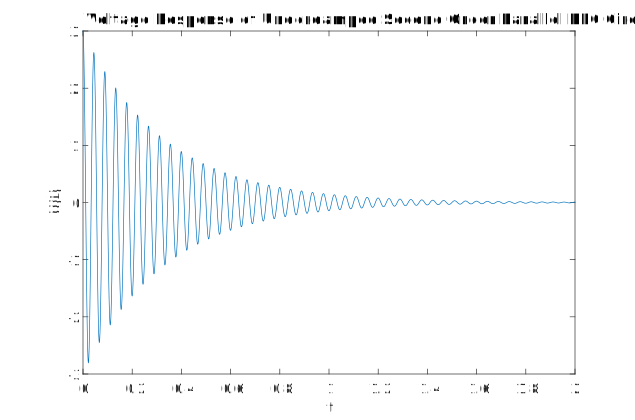
\includegraphics[scale=0.6]{plot4_1.png}
\end{figure}

The above figure shows the correct behavior of an underdamped RLC circuit as it shows $v(t)$ oscillating between above and below steady state value before settling down at steady state value.

%2
\section{Overdamped Second Order Parallel RLC Circuit}
\begin{center}
    \begin{circuitikz}
        \draw 
            (0,0) -- (-2,0) to[voltage source, l_= $V_s$] (-2,-3) -- (0,-3)
            (0,0) 
            coordinate(R1) -- ++(2.25,0)
            coordinate(n1) -- ++(1.75,0)
            coordinate(L1) -- ++(1.75,0)
            coordinate(n2) -- ++(2.25,0)
            coordinate(C1)
            (R1) to[R=$R\equal\SI{50}{\ohm}$, i>^=$i_R$] ++(0,-3)
            (n1) ++(0,-0.25) to[open, v^=v] ++(0,-2.5)
            (L1) node[circ,label=v]{} to[L=$L\equal\SI{1}{\henry}$, i>^=$i_L\equal I_0$] ++(0,-3) node[ground]{}
            (n2) ++(0,-0.25) to[open, v^=v] ++(0,-2.5)
            (C1) to[C=$C\equal\SI{50}{\micro\farad}$, i>^=$i_c$, v=$v_c$] ++(0,-3) --(0,-3)
            ;
    \end{circuitikz}
\end{center}

The voltage response of the above RLC circuit can be represented by the differential equation below:

$$\frac{d^2v}{dt^2}+\frac{1}{RC}\frac{dv}{dt}+\frac{1}{LC}v=0$$

The damping factor $\alpha$ and undamped natural frequency $\omega_0$ for the above parallel RLC circuit is the following:
$$\alpha = \frac{1}{2RC}$$
$$\omega_0 = \sqrt{\frac{1}{LC}}$$\\

The condition for solution in underdamped, critically damped, and overdamped case in terms of $\alpha$ and $\omega_0$ is the following:
\[ \begin{cases} 
      \alpha < \omega_0 & underdamped \\
      \alpha = \omega_0 & critically\; damped \\
      \alpha > \omega_0 & overdamped 
   \end{cases}
\]\\

For the RLC circuit to be overdamped, the below inequality must be satisfied:
$$\alpha > \omega_0$$
$$\frac{1}{2RC}>\sqrt{\frac{1}{LC}}$$
$$2RC<\sqrt{LC}$$
$$R<\sqrt{\frac{L}{4C}}\approx\SI{70.71}{\ohm}$$\\

$R_{OD}=\SI{50}{\ohm}$ was used for the following calculations for an overdamped RLC circuit.\\

The damping factor $\alpha$, undamped natural frequency $\omega_0$ and damped natural frequency for the above parallel RLC circuit is the following:
$$\alpha = \frac{1}{2RC}=200$$
$$\omega_0 = \sqrt{\frac{1}{LC}}=\approx 141.42$$
$$\omega_d=\sqrt{\alpha^2-\omega_0^2}\approx 141.42$$\\

The characteristic equation in relation to the above differential equation is the following:
$$s^2+2\alpha s+\omega_0^2=0$$\\

Utilizing the quadratic equation, we can obtain the following expressions for determining the roots of the characteristic equation in terms of RLC and in terms of $\alpha$ and $\omega_0$:
$$s=-\alpha \pm\omega_d$$
$$s_1=-\alpha +\omega_d\approx-58.58$$
$$s_2=-\alpha -\omega_d\approx-341.42$$

The general solution of v(t) is as follows:
$$v(t)=A_1e^{s_1t}+A_2e^{s_2t}$$

The initial condition v'(0) can be determined as follow with KCL at node v:
$$i_R+i_L+i_c=0$$
$$\frac{v}{R}+I_0+Cv'=0$$
$$v'=-\frac{\frac{v}{R}+I_0}{C}$$
$$v'(0)=-\frac{\frac{v(0)}{R}+I_0}{C}=-1200$$\\

The coefficient $A_1$ and $A_2$ can be calculated based on initial condition $v(0)$ and $v'(0)$ as follows:
$$v(0) = A_1e^{s_10} + A_2e^{s_20} = A_1 + A_2$$
$$v'(0) = A_1s_1e^{s_10} + A_2s_2e^{s_20}$$
$$v'(0) = s_1A_1 + s_2A_2$$

$$
\begin{bmatrix}
1 & 1 \\
s_1 & s_2 
\end{bmatrix}
\begin{bmatrix}
A_1\\
A_2
\end{bmatrix}
=
\begin{bmatrix}
v(0)\\
v'(0)
\end{bmatrix}
$$

$$A_1 = \frac{s_2v(0)-v'(0)}{s_2-s_1} = -0.6213$$
$$A_2 = v(0)-A_1 = 3.6213$$

The complete solution of v is the following:
$$v(t)=-0.6213e^{-58.58t}+3.6213e^{-341.42t}$$

The following is the plot of $v(t)$ with MATLAB. The source code is appended at the end of this report.
\begin{figure}[H]
    \centering
        \includegraphics[scale=0.6]{plot4_2.png}
\end{figure}

The above figure shows the correct behavior of an overdamped RLC circuit as unlike in the underdamped case, instead of oscillating above and below the steady state value, it shows $v(t)$ reaching from above to below steady state value once and only once before settle down at steady state value. The much lower resistor value results in a much higher damping factor, therefore force the circuit to settle in place much faster.



\end{document}